\section{Questions sur le chapitre ``Turbines à gaz et cycles à vapeurs''}
\subsection{Dessinez un cycle thermodynamique idéal d'une turbine à gaz sur les plans $(p,v)$ et $(T,s)$. Décrivez les 4 étapes du cycle.}
Le cycle de Brayton, aussi connu sous le nom de cycle de Joule, est le cycle idéal correspondant à la turbine à gaz élémentaire. Il existe deux types de cycles de Brayton selon qu'il soit ouvert, ou refermé sur l'atmosphère en utilisant un échangeur de chaleur. C'est la première variante qui retiendra notre attention puisque c'est celle qui est utilisée dans les centrales électriques Turbines Gaz Vapeurs (TGV). Le cycle est constitué de quatre étapes (voir Figure \ref{fig:cycleTG}):
\begin{description}
	\item[1 $\rightarrow$ $\mathbf{2_S}$] Compression de l'air au moyen d'un compresseur.
	\item[$\mathbf{2_S}$ $\rightarrow$ 3] L'air comprimé est chauffé dans la chambre de combustion lors d'un processus isobare.
	\item[3 $\rightarrow$ $\mathbf{4_S}$] Détente des fumées au moyen d'une turbine.
	\item[$\mathbf{4_S}$ $\rightarrow$ 1] Rejet des fumées dans l'atmosphère.
\end{description} 
Compresseur, turbine et alternateur sont sur le même arbre. C'est donc la turbine qui entraîne le compresseur at l'alternateur. Dans un cycle idéal, la compression et la détente sont supposées isentropiques tandis que la combustion est supposée isobare.
\begin{figure}[p]\centering 
	\tikzsetnextfilename{cycleTG}
	\begin{tikzpicture}
		\draw[top color=gray!10, bottom color=gray!90] (1.5,{1.4+1.5*sin(15)}) rectangle (7.5,{1.6+1.5*sin(15)});
		\draw[-triangle 45,red,thick] (0,0) -- (0,1);
		\draw[fill=gray!30] (-0.5,{1-0.5*sin(15)}) -- ++(2,{2*sin(15)}) -- ++(0,1) -- ++(-2,{2*sin(15)}) --cycle;
		\draw[-triangle 45,red,thick] (1,{2+2*sin(15)}) |- ++(1,1) coordinate (A);
		\draw[-triangle 45,red,thick] (1,{3.5+2*sin(15)}) -- (2,{3.5+2*sin(15)}); 
		\draw[fill=gray!30] (A) -- ++(0,1) -- ++(2.5,0) -- ++(0,-1) coordinate (B) -- ++(0,-0.5) -- ++(-2.5,0) --cycle;
		\draw[-triangle 45,red,thick] (B) -| ++(1,-1) coordinate (C);
		\draw[fill=gray!30] (C) -- ++(-0.5,-{0.5*sin(15)}) -- ++(0,-1) -- ++(1.5,{-1.5*sin(15)}) coordinate (D) -- ++(0.5,{-0.5*sin(15)}) -- ++(0,2) --cycle;
		\draw[-triangle 45,red,thick] (D) -- ++(0,-1);
		\draw (-0.5,0.3) node[draw,circle]{1};
		\draw (0,0.3) node{--};
		\draw (0,0) node[below]{\small Air};
		\draw (0.5,{1.5+1.5*sin(15)}) node{\small Compresseur};
		\draw (1.5,{2+2*sin(15)+0.3}) node[draw,circle]{2};
		\draw (1,{2+2*sin(15)+0.3}) node{--};
		\draw (1,{3.5+2*sin(15)}) node[left]{\small Combustible};
		\draw (3.25,{3.25+2*sin(15)}) node{\small Combustion};
		\draw (5,{3+2*sin(15)+0.5}) node[draw,circle]{3};
		\draw (5,{3+2*sin(15)}) node[rotate=90]{--};
		\draw (6,{1.5+1.5*sin(15)}) node{\small Turbine};
		\draw (6.5,0.5) node{--};
		\draw (7,0.5) node[draw,circle]{4};
		\draw (6.5,0) node[below]{\small Fumées};
		\draw[-latex] (3.25,{1.75+1.5*sin(15)}) arc (30:330:0.25 and 0.5);
	\end{tikzpicture}
	\tikzsetnextfilename{pvcycleTG}
    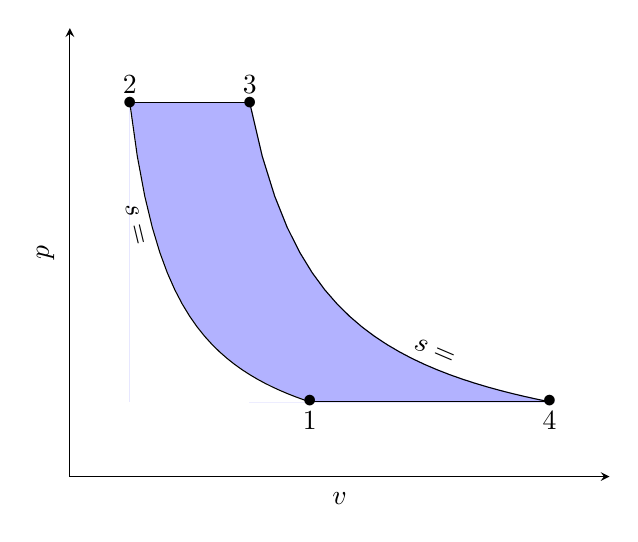
\begin{tikzpicture}
        \begin{axis}[%
    		enlargelimits=true,
        	grid=none,
        	axis lines=left, xtick=\empty, ytick=\empty,
        	xmin = 0, xmax = 9,
        	ymin = -1, ymax = 5,
        	ylabel=$p$,
        	xlabel=$v$,
        	no markers,
        ]        	
        	\addplot+[domain=1:3,fill,blue!30] { 4 } \closedcycle;
        	\addplot+[domain=3:8,fill,blue!30] { 6.25/(x-1.75) - 1} \closedcycle;
        	\addplot+[domain=1:4,fill,white] { 3.75/(x-0.25) - 1 } \closedcycle;
        	\addplot+[domain=4:8,fill,white] { 0 } \closedcycle;
        	\addplot[domain=1:3] { 4 };
        	\addplot[domain=3:8] { 6.25/(x-1.75) - 1 } node[pos=0.7,sloped,above]{$s=\constant$};
        	\addplot[domain=1:4] { 3.75/(x-0.25) - 1 } node[pos=0.3,sloped,below]{$s=\constant$};;
        	\addplot[domain=4:8] { 0 };
        	
        	\draw (4,0) node{$\bullet$} node[below]{1};
        	\draw (1,4) node{$\bullet$} node[above]{2};
        	\draw (3,4) node{$\bullet$} node[above]{3};
        	\draw (8,0) node{$\bullet$} node[below]{4};
    	\end{axis}
    \end{tikzpicture}
    \tikzsetnextfilename{TScycleTG}
    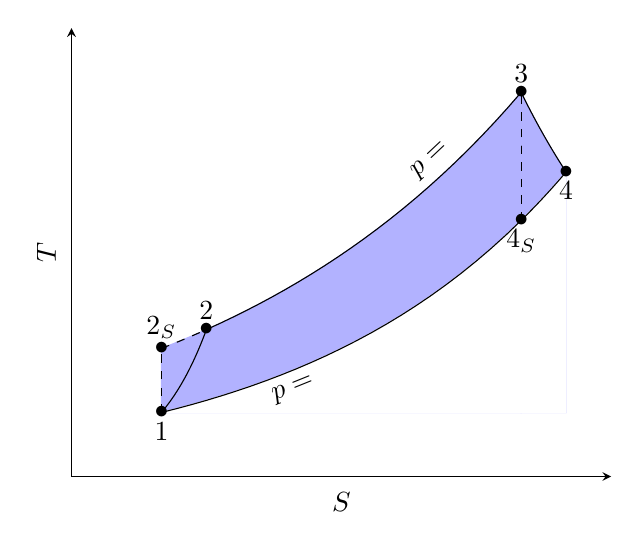
\begin{tikzpicture}
        \begin{axis}[%
    		enlargelimits=true,
        	grid=none,
        	axis lines=left, xtick=\empty, ytick=\empty,
        	xmin = 0, xmax = 6,
        	ymin = -1, ymax = 6,
        	ylabel=$T$,
        	xlabel=$S$,
        	no markers,
        ]        	
        	\addplot+[domain=1:5,fill,blue!30] { 1.5197*1.3161^x - 1 } \closedcycle;
        	\addplot+[domain=5:5.5,fill,blue!30] { 87.1945*0.5645^x } \closedcycle;
        	\addplot+[domain=1:5.5,fill,white] { 0.7071*1.4142^x - 1 } \closedcycle;
        	\addplot[dashed,domain=0:1] (1,x);
        	\addplot[dashed,domain=1:1.5] { 1.5197*1.3161^x - 1 };
        	\addplot[domain=1.5:5] { 1.5197*1.3161^x - 1 } node[pos=0.7,sloped,above]{$p=\constant$};
        	\addplot[domain=5:5.5] { 87.1945*0.5645^x };
        	\addplot[domain=1:5] { 0.7071*1.4142^x - 1 } node[pos=0.3,sloped,below]{$p=\constant$};
        	\addplot[domain=5:5.5] { 0.7071*1.4142^x - 1 };
        	\addplot[domain=1:1.5] { 0.1899*5.2647^x - 1 };
        	\addplot[dashed,domain=3:5] (5,x);
        	
        	\draw (1,0) node{$\bullet$} node[below]{1};
        	\draw (1,1) node{$\bullet$} node[above]{$2_S$};
        	\draw (1.5,1.2945) node{$\bullet$} node[above]{2};
        	\draw (5,3) node{$\bullet$} node[below]{$4_S$};
        	\draw (5.5,3.7568) node{$\bullet$} node[below]{$4$};
        	\draw (5,5) node{$\bullet$} node[above]{3};
    	\end{axis}
    \end{tikzpicture}
	\caption{Schéma de principe et diagrammes ($p$,$v$) et ($T$,$S$) d'une turbine à gaz}
	\label{fig:cycleTG}
\end{figure}

\subsection{On considère le cycle d'une turbine à gaz. On suppose que $p_2 = p_3$, que $c_p = C^\text{te}$ et que les flux de masse à la turbine et au compresseur sont égaux. Dérivez l'expression du rendement thermique du cycle.}
L'expansion thermique des gaz due à l'effet de la source chaude donne lieu à la production d'une puissance motrice de détente supérieure à celle nécessaire à la compression du gaz frais. La puissance effective $P_e$ de cette installation peut s'écrire :
\begin{equation} P_e = \underbrace{P_{mT}}_{\text{turbine}} - \underbrace{P_{mC}}_{\text{compresseur}} - \underbrace{P_{fm+aux}}_{\text{frottements mécaniques et auxilliaires}} \end{equation} 
En désignant $\dot{m}_T$ et $\dot{m}_C$ les flux de masse à la turbine et au compresseur, il vient encore :
\begin{equation} P_e = \dot{m}_TW_{mT} - \dot{m}_CW_{mC} - P_{fm+aux} \end{equation}
On peut donc définir la puissance motrice 
\begin{equation} P_m = P_e + P_{fm+aux} = \dot{m}_TW_{mT} - \dot{m}_CW_{mC} \end{equation}
Le travail moteur de l'installation s'exprime donc :
\begin{equation} W_m = \frac{P_m}{\dot{m}_C} = \frac{\dot{m}_T}{\dot{m}_C}W_{mT}-W_{mC} \end{equation}
En prenant en compte les hypothèses simplificatrices habituelles d'identité des états d'énergie cinétique et d'énergie potentielle en chacun des point remarquables du cycle ($\Delta k = \Delta z = 0$) ainsi que le caractère adiabatique des transformations de compression et de détente, nous obtenons :
\begin{align} W_{mT} &= -\int^4_3vdp - W_{fT} = h_3-h_4 \\ W_{mC} &= \int^2_1vdp + W_{fC} = h_2-h_1 \end{align}
Étant donné que les flux de masse à la turbine et au compresseur sont égaux ($\dot{m}_T = \dot{m}_C$), que $c_p$ est constant et que $p_2 = p_3$, le travail moteur s'écrit  
\begin{equation} W_m = (h_3-h_4) - (h_2-h_1) = c_p\left((T_3-T_4) - (T_2-T_1)\right)\end{equation}
Avec toutes les hypothèses, la chaleur fournie lors de la combustion $Q$ correspond à 
\begin{equation} Q = \Delta^3_2h \end{equation}
On trouve donc l'expression du rendement thermique du cycle :
\begin{equation} \eta_{th} = \frac{W_m}{Q} = \frac{c_p((T_3-T_4)-(T_2-T_1))}{c_p(T_3-T_2)} = \frac{T_3-T_2-T_4+T_1}{T_3-T_2} = 1 - \frac{T_4-T_1}{T_3-T_2} \label{eq:q4_3}\end{equation}

\newcommand{\sit}{\eta_\text{SiT}}
\newcommand{\sic}{\eta_\text{SiC}}
\subsection{À partir de l'expression \ref{eq:q4_3}, dérivez l'expression du rendement thermique $\eta_\text{th}$ d'une turbine à gaz en fonction du rendement isentropique interne $\sic$ du compresseur et $\sit$ de la turbine.} 
L'introduction des notions de rendement isentropique interne $\sic$ de la compression et $\sit$ de la turbine nous permet de réécrire l'équation du travail moteur :
\begin{align} W_m &= \sit c_p(T_3-T_{4S})-\frac{1}{\sic}c_p(T_{2S}-T_1) \\ &= \sit c_pT_3\left(1-\frac{T_{4S}}{T_3}\right)-\frac{1}{\sic}c_pT_1\left(\frac{T_{2S}}{T_1}-1\right)\end{align}
et celle de l'effet calorifique fourni par la combustion :
\begin{align} Q_I &= c_p(T_3-T_2) \\ &= c_p(T_3-(T_2-T_1)-T_1) \\ &= c_p\left(T_3-T_1-\frac{1}{\sic}(T_{2S}-T_1)\right) \end{align}
Les états $2S$ et $4S$ sont ceux qui seraient atteint respectivement en fin de compression et de détente adiabatiques sans travaux dissipatifs (voir figure \ref{fig:cycleTG}). Pour simplifier l'écriture, on pose :
\begin{equation} X \triangleq \left(\frac{p_2}{p_1}\right)^{\frac{\gamma-1}{\gamma}} = \left(\frac{p_3}{p_4}\right)^{\frac{\gamma-1}{\gamma}} = \frac{T_{2S}}{T_1} = \frac{T_3}{T_{4S}} \label{eq:Xcomp}\end{equation}
qui est une image non linéaire du rapport de pression réalisé dans la machine. On introduit aussi le rapport entre la température maximale du fluide moteur et la température de base du cycle\footnote{On exprime par ce paramètre $Y$ la contrainte thermique à laquelle sera astreinte la turbine. Il est impératif de conserver à chaud la tenue mécanique et les qualités aérodynamiques des ailettes, ce qui conduit à limiter $T_3$ en pratiquant pour la combustion un coefficient d'excès d'air adéquat.} , à savoir :
\begin{equation} Y \triangleq \frac{T_3}{T_1} \label{eq:Ytemp}\end{equation} 
L'utilisation des paramètres $X$ et $Y$ conduit aux relations adimensionnelles :
\begin{align} \frac{W_m}{c_pT_1} &= \sit Y\left(1-\frac{1}{X}\right) - \frac{1}{\sic}\left(X-1\right) \\ &= \left(\sit\frac{Y}{X}-\frac{1}{\sic}\right)(X-1) \end{align}
et 
\begin{align} \frac{Q_I}{c_pT_1} &= Y - 1 - \frac{1}{\sic}(X-1) \end{align} 
On tire de ces expressions celle du rendement thermique $\eta_{th}$ en fonction de $\sic$ et $\sit$:
\begin{equation} \eta_{th} = \frac{W_m}{Q_I} = \frac{\left(\sit\frac{Y}{X}-\frac{1}{\sic}\right)(X-1)}{Y - 1 - \frac{1}{\sic}(X-1)} \end{equation}

\newcommand{\pit}{\eta_\text{piT}}
\newcommand{\pic}{\eta_\text{piC}}
\subsection{À partir de l'expression \ref{eq:q4_3}, dérivez l'expression du rendement thermique $\eta_\text{th}$ d'une turbine à gaz en fonction du rendement polytropique $\pic$ du compresseur et $\pit$ de la turbine.\label{q:9.4}}
On réécrit l'équation du travail moteur :
\begin{equation} W_m = c_pT_3\left(1-\frac{T_4}{T_3}\right) - c_pT_1\left(\frac{T_2}{T_1}-1\right) \end{equation}
et celle de l'effet calorifique fourni par la combustion :
\begin{equation} Q_I = c_pT_1\left(\frac{T_3}{T_1}-\frac{T_2}{T_1}\right)\end{equation}
Le recours au modéle polytropique du fonctionnement des turbomachines pour décrire les transformation qui s'y produisent avec travaux dissipatifs $W_f$ conduit à utiliser les rendements polytropiques $\pic$ du compresseur et $\pit$ de la turbine tels que l'on ait :
\begin{align} \frac{T_2}{T_1} &= \left(\frac{p_2}{p_1}\right)^{\frac{m-1}{m}} = \left(\frac{p_2}{p_1}\right)^{\frac{\gamma-1}{\gamma}\frac{1}{\pic}} = \left(\frac{T_{2S}}{T_1}\right)^{\frac{1}{\pic}} = X^{\frac{1}{\pic}} \\ \frac{T_4}{T_3} &= \left(\frac{p_4}{p_3}\right)^{\frac{m-1}{m}} = \left(\frac{p_4}{p_3}\right)^{\frac{\gamma-1}{\gamma}\pit} = \left(\frac{T_{4S}}{T_3}\right)^{\pit} = \left(\frac{1}{X}\right)^{\pit} \end{align}
avec $m$ l'indice polytropique, $\gamma$ l'indice adiabatique, $T_{2S}$ et $T_{4S}$ les températures aux états $2S$ et $4S$ qui seraient atteint respectivement en fin de compression et de détente adiabatiques sans travaux dissipatifs $W_f$ et $X$ l'image non linéaire du rapport de pression réalisé dans la machine défini par l'équation \ref{eq:Xcomp}. On conserve le paramètre $Y$ défini par l'équation \ref{eq:Ytemp}. L'utilisation des paramètres $X$ et $Y$ conduit aux relations adimensionnelles :
\begin{align} \frac{W_m}{c_pT_1} &= Y\left(1-\frac{1}{X^{\pit}}\right) - X^{\frac{1}{\pic}} + 1 \\ \frac{Q_I}{c_pT_1} &= Y - X^{\frac{1}{\pic}} \end{align}
On tire de ces expression celle du rendement thermique $\eta_{th}$ en fonction de $\pic$ et $\pit$ :
\begin{equation} \eta_{th} = \frac{W_m}{Q_I} = \frac{Y\left(1-\frac{1}{X^{\pit}}\right) - X^{\frac{1}{\pic}} + 1}{Y - X^{\frac{1}{\pic}}} \end{equation}


\subsection{À partir de l'expression \ref{eq:q4_5}, dérivez l'expression du travail moteur $W_m$ d'une turbine à gaz en fonction du rendement isentropique interne $\eta_\text{SiC}$ du compresseur et $\eta_\text{SiT}$ de la turbine. Pour un rapport de température \ref{eq:q4_52} fixé, calculer les valeurs du rapport de compression \ref{eq:q4_53} qui annulent $W_m$.}
\begin{equation} \label{eq:q4_5} W_m = c_p\left(\left(T_3-T_4\right) - \left(T_2-T_1\right)\right) \end{equation}
\begin{equation} \label{eq:q4_52} Y = \frac{T_3}{T_1} \end{equation}
\begin{equation} \label{eq:q4_53} X = \left(\frac{p_2}{p_1}\right)^\frac{(\gamma-1)}{\gamma} \end{equation}

On peut réécrire l'équation \ref{eq:q4_5} en y introduisant les rendements isentropiques internes des turbomachines :
\begin{equation} W_m = c_pT_3\left(1-\frac{T_4}{T_3}\right) - c_pT_1\left(\frac{T_2}{T_1} - 1\right) = \sit c_pT_3\left(1-\frac{T_{4S}}{T_3}\right) - \frac{1}{\sic}c_pT_1\left(\frac{T_{2S}}{T_1} - 1\right) \end{equation}
Le paramètre $X$ peut aussi s'écrire :
\begin{equation} X \triangleq \left(\frac{p_2}{p_1}\right)^\frac{(\gamma-1)}{\gamma} = \frac{T_3}{T_{4S}} = \frac{T_{2S}}{T_{1}} \end{equation}
On a donc :
\begin{equation} \frac{W_m}{c_pT_1} = \left(\sit\frac{Y}{X}-\frac{1}{\sic}\right)(X-1) \end{equation}
On observe que le travail moteur s'annulent en $X=1$ et en $X = X_0$ de valeur :
\begin{equation} X_0 = \sic\sit Y \end{equation}

\subsection{À partir de l'expression \ref{eq:q4_5}, dérivez l'expression du travail moteur $W_m$ d'une turbine à gaz en fonction du rendement polytropique $\eta_\text{piC}$ du compresseur et $\eta_\text{piT}$ de la turbine. Dérivez également le maximum de $W_m$ en fonction du rapport de compression \ref{eq:q4_53}.}
L'étape de dérivation de l'expression du travail moteur $W_m$ en fonction des rendements polytropiques $\pic$ et $\pit$ a déjà été développée à la section \ref{q:9.4} :
\begin{equation} \frac{W_m}{c_pT_1} = Y\left(1-\frac{1}{X^{\pit}}\right) - X^{\frac{1}{\pic}} + 1 \end{equation}
On trouve la valeur maximale de $W_m$ selon $X$ en annulant sa dérivée selon $X$ :
\begin{align} \fpart{}{X}\left(Y\left(1-\frac{1}{X^{\pit}}\right) - X^{\frac{1}{\pic}} + 1\right) &= 0 \\ \pit YX^{-\pit-1} - \frac{X^{\frac{1}{\pic}-1}}{\pic} &= 0 \\ X^{\pit+\frac{1}{\pic}} &= \pit\pic Y \\ X_A &= \left(\pit\pic Y\right)^{\frac{1}{\frac{1}{\pic}+\pit}} \simeq \sqrt{\pit\pic Y} \end{align}
où $X_A$ correspond à la valeur pour laquelle $W_m$ passe par un maximum. On remarque que $X_A$ est une fonction croissante de $Y$.


\subsection{Dans l'utilisation des turbines à gaz essaye-t-on de maximiser le travail effectif, $W_e$, ou le rendement effectif, $\eta_e$. Justifiez votre réponse.}
On rappelle que le rendement effectif est défini par $\eta_e \triangleq \eta_{th}\eta_{mec}$ et le travail effectif par $W_e \triangleq \eta_{mec}W_m$.
Soit $X_A$ le rapport de compression qui maximise le travail moteur et $X_B$ celui qui maximise le rendement thermique. Le maximum du rendement effectif correspond à une valeur $X_M$ telle que l'on ait toujours :
\begin{equation} X_A \leq X_M \leq X_B \end{equation} 
On observe en pratique que :
\begin{itemize}
\item la variation relative du rendement effectif est moindre que celle du travail effectif dans l'intervalle $X_A \leq X_M \leq X_B$. Il est donc plus pénalisant pour le travail effectif de choisir le point $X_B$ qu'il n'est pénalisant pour le rendement de choisir le point $X_A$;
\item en termes de rapport de pression, le fonctionnement à rendement maximum est de loin plus exigeant que le fonctionnement à travail moteur maximum et implique le recours à une technologie plus coûteuse tant pour le compresseur (nombre élevé d'étages) que pour la chambre de combustion (haute densité de puissance thermique).
\end{itemize}
On utilisera donc en pratique un rapport de compression plus proche de celui donnant lieu au maximum de travail que celui conduisant au maximum du rendement.

\subsection{Donnez la définition d'exergie dans une installation à cycle combiné et expliquez sa signification physique.}
Une installation à cycle combiné profite de la température encore élevée des gaz d'échappement pour produire du travail moteur par un cycle thermique en aval de la turbine à gaz. En pratique il s'agit d'un cycle utilisant la détente dans une turbine de la vapeur sous pression produite par une chaudière grâce à la récupération d'une fraction de l'enthalpie sensible des gaz d'échappement (voir exemple figure \ref{fig:cycleTGCAV}). Si l'on désigne par $\eta_R$ le taux de récupération de cette enthalpie sensible, qui représente pour la turbine à gaz la perte à la source froid $1-\eta_{TG}$, tandis que $\eta_{CAV}$ désigne le rendement de conversion en travail de la chaleur ainsi récupérée, le rendement global de conversion de la chaleur en travail moteur a pour valeur dans une installation combinée :
\begin{equation} \eta_{TGCAV} = \eta_{TG} + (1-\eta_{TG})\eta_R\eta_{CAV} \label{eq:eta_TGCAV}\end{equation}
Il est possible de situer le potentiel et les limites du rendement en faisant usage de la notion d'exergie. L'exergie est la fonction d'état définie par la relation 
\begin{equation} e \triangleq (H-H_1)-T_1(S-S_1) \end{equation}
et qui représente le travail maximum que l'on peut obtenir d'un fluide du fait de sont état de déséquilibre par rapport au conditions de l'ambiance, considérée comme source froide infinie à température $T_1$ et pression $p_1$.
\begin{figure}[p]\centering
	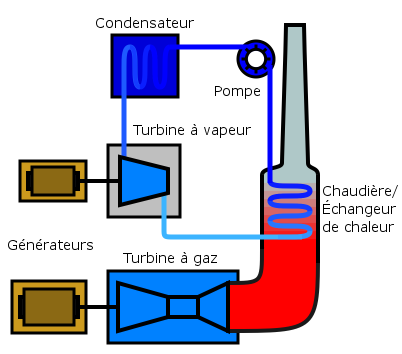
\includegraphics{figures/cycleTGCAV}	
	\caption{Exemple d'une installation à cycle combiné\label{fig:cycleTGCAV}}
\end{figure}

\subsection{Dérivez l'expression du rendement global $\eta_\text{TGCAV}$ d'un cycle combiné en fonction des températures des sommets du cycle.}
Pour obtenir le maximum de travail moteur des gaz d'échappement, on peut imaginer de les détendre de façon adiabatique et sans travaux dissipatifs de leur état initial 4 à un état final 5 d'entropie $S_4 = S_5$ et de température $T_5=T_1$, la pression $p_5$ étant dès lors bien inférieure à celle $p_1$ (voir diagramme $(T,S)$ figure \ref{fig:TScycleTGCAV}). Cette détente idéale produirait un travail moteur
\begin{equation} W_{mD} = H_4-H_1 \end{equation}
Afin de pouvoir rejeter dans l'atmosphère le fluide ainsi détendu, il faudrait alors le comprimer de $p_5$ à $p_1$, et consentir pour cela la consommation d'un travail moteur dont le miminum correspond à une compression isotherme utilisant l'atmosphère de température $T_1$ comme source froide. Le travail de compression aurait alors pour valeur 
\begin{equation} W_{mC} = T_1(S_4-S_1) \end{equation}
Ceci montre que l'exergie est bien le travail moteur maximum récupérable sur l'énergie disponibles des gaz d'échappement. Le rendement de conversion en travail de l'enthalpie sensible de ces gaz a donc pour valeur :
\begin{align} \eta_{CAV} &= \frac{W_{mD}-W_{mC}}{W_{mD}} \\ &= \frac{H_4-H_1-T_1(S_4-S_1)}{H_4-H_1} \\ &= \frac{c_p(T_4-T_1) - T_1c_p\ln\left(\frac{T_4}{T_1}\right)}{c_p(T_4-T_1)} \\ &= 1 - \frac{T_1}{T_4-T_1}\ln\left(\frac{T_4}{T_1}\right) \end{align}
En introduisant l'expression \ref{eq:q4_3} du rendement thermique du cycle de la turbine à gaz dans l'expression \ref{eq:eta_TGCAV} du rendement global on obtient :
\begin{equation} \eta_{TGCAV} = 1 - \frac{T_4-T_1}{T_3-T_2} + \frac{T_4-T_1}{T_3-T_2}\left(1-\frac{T_1}{T_4-T_1}\ln\left(\frac{T_4}{T_1}\right)\right) \end{equation}
Soit finalement :
\begin{equation} \eta_{TGCAV} = 1-\frac{T_1}{T_3-T_2}\ln\left(\frac{T_4}{T_1}\right) \end{equation}
\begin{figure}[p]\centering
	\tikzsetnextfilename{TScycleTGCAV}
    \begin{tikzpicture}
        \begin{axis}[%
    		enlargelimits=true,
        	grid=none,
        	axis lines=left, xtick=\empty, ytick=\empty,
        	xmin = 0, xmax = 6,
        	ymin = -1, ymax = 6,
        	ylabel=$T$,
        	xlabel=$S$,
        	no markers,
        ]        	
        	%\addplot+[domain=1:1.5,fill,blue!30] { 0.1899*5.2647^x - 1 } \closedcycle;
        	%\addplot+[domain=1.5:5,fill,blue!30] { 1.5197*1.3161^x - 1 } \closedcycle;
        	%\addplot+[domain=5:5.5,fill,blue!30] { 87.1945*0.5645^x } \closedcycle;
        	%\addplot+[domain=1:5.5,fill,white] { 0.7071*1.4142^x - 1 } \closedcycle;
        	%\addplot[dashed,domain=0:1] (1,x);
        	%\addplot[dashed,domain=1:1.5] { 1.5197*1.3161^x - 1 };
        	\addplot[black!50,domain=0.5:5.5] { 1.5197*1.3161^x - 1 } node[pos=0.5,sloped,above]{$p=\constant$};
        	\addplot[black!50,domain=0.5:6] { 0.7071*1.4142^x - 1 } node[pos=0.4,sloped,below]{$p=\constant$};
        	\addplot[domain=1.5:5] { 1.5197*1.3161^x - 1 };
        	\addplot[domain=5:5.5] { 87.1945*0.5645^x };
        	\addplot[domain=0:3.7568] (5.5,x);
        	\addplot[domain=1:5.5] {0};
        	%\addplot[domain=1:5.5] { 0.7071*1.4142^x - 1 };
        	\addplot[domain=1:1.5] { 0.1899*5.2647^x - 1 };
        	%\addplot[dashed,domain=3:5] (5,x);
        	
        	\draw (1,0) node{$\bullet$} node[below]{1};
        	%\draw (1,1) node{$\bullet$} node[above]{$2_S$};
        	\draw (1.5,1.2945) node{$\bullet$} node[above]{2};
        	%\draw (5,3) node{$\bullet$} node[below]{$4_S$};
        	\draw (5.5,3.7568) node{$\bullet$} node[right]{$4$};
        	\draw (5.5,0) node{$\bullet$} node[right]{$5$};
        	\draw (5,5) node{$\bullet$} node[above]{3};
    	\end{axis}
    \end{tikzpicture}
    \caption{Diagramme $(T,S)$ d'une installation à cycle combiné} 
    \label{fig:TScycleTGCAV}
\end{figure}

\subsection{Dérivez l'expression du rendement propulsif $\eta_P$ d'une turbine à gaz qui est utilisée en propulsion aérienne.}
Une turbine à gaz utilisée en propulsion aérienne crée la poussée $F$ destinée à compenser la traînée de l'avion et à lui conserver sa vitesse, par effet de réaction de l'air qui, s'approchant de l'avion à vitesse $c$ (dans un repère lié à l'avion), s'en éloigne à vitesse $c_s > c$ grâce à l'action du système propulsif. Pour un débit $\dot{m}$ passant dans le système propulsif, la relation fondamentale sur la conservation du flux de quantité de mouvement s'écrit :
\begin{equation} F = \dot{m}(c_s-c) \end{equation}
On définit la puissance propulsive par le produit de la poussée avec la vitesse de vol :
\begin{equation} P_p \triangleq Fc = \dot{m}(c_s-c)c \end{equation}
tandis que la puissance motrice dépensée résulte de la variation de l'énergie cinétique de l'air propulseur et a pour valeur :
\begin{equation} P_m = \dot{m}(\Delta K + W_f) \end{equation}
On exprime $W_f$ par une fraction de l'énergie cinétique de l'air qui transite dans le propulseur :
\begin{equation} W_f = (\xi-1)\frac{c_s^2}{2} \qquad \text{avec} \qquad \xi\geq 1 \end{equation}
et
\begin{equation} \Delta K = \frac{c_s^2-c^2}{2} \end{equation}
La puissance motrice s'écrit alors :
\begin{equation} P_m = \dot{m}\frac{\xi c_s^2-c^2}{2} \end{equation}
Le rendement propulsif a donc pour valeur :
\begin{equation} \eta_P = \frac{P_p}{P_m} = 2\frac{(c_s-c)c}{\xi c_s^2-c^2}  = 2\frac{\frac{c_s}{c}-1}{\xi\frac{c_s^2}{c^2}-1} \end{equation}
On voit que le rendement est fonction du rapport de vitesse et est optimum lorsque ce rapport a pour valeur :
\begin{equation} \frac{c_s}{c} = 1 + \sqrt{1-\frac{1}{\xi}} \end{equation}
À cette valeur, toujours inférieure à 2, correspond le rendement propulsif optimum de valeur :
\begin{equation} \eta_{P,max} = \frac{1}{\xi+\sqrt{\xi(\xi-1)}} \end{equation}

\subsection{Décrivez les avantages technologiques des turbines à gaz dans leur utilisation en propulsion aérienne et marine.}
Propulsion aérienne
\begin{itemize}
\item Le rapport puissance/masse de la turbine à gaz en fait le moteur idéalement compact pour la propulsion des avions.
\item La turbine à gaz répond à l'exigence d'une grande fiabilité mécanique liée à la relative simplicité de la maintenance.
\item La turbine à gaz dispose de grandes puissances unitaires pour voler vite et à haute altitude.
\item La diminution de $\rho_\text{air}$ ne constitue pas un handicap comparable à celui subi par les moteurs volumétriques.
\item L'abaissement de la température ambiante est très favorable au rendement par l'effet important qu'il a sur le rapport $Y = T_3/T_1$.
\end{itemize}

Propulsion marine 
\begin{itemize}
\item Le démarrage de l'ensemble rotorique est indépendant de l'actionnement du système propulsif.
\item La compacité d'une turbine à gaz
\end{itemize}
